\documentclass[tikz,border=4pt]{standalone}
\usepackage{amsmath}
\usetikzlibrary{patterns}
\begin{document}
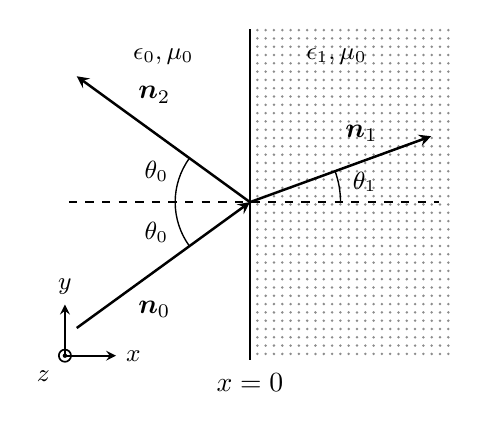
\begin{tikzpicture}[>=stealth, thick, scale=1.0]
  % Dielectric region x > 0
  \fill[pattern=dots, pattern color=black!45] (0, -2.0) rectangle (2.6, 2.2);

  % Interface x = 0
  \draw[line width=0.9pt] (0, -2.0) -- (0, 2.2);
  \node[below] at (0, -2.05) {$x = 0$};

  % Normal line along y = 0
  \draw[dashed, line width=0.55pt] (-2.3, 0) -- (2.4, 0);

  % Incident ray n0 (theta0 = 36 deg from +x in x < 0, going up-right)
  \draw[->, line width=0.9pt] (-2.2, {-2.2*tan(36)}) -- (0, 0);
  \node[below right] at (-1.55, {-1.55*tan(36)}) {$\boldsymbol{n}_0$};

  % Reflected ray n2 (angle 36 deg above -x, going up-left)
  \draw[->, line width=0.9pt] (0, 0) -- (-2.2, {2.2*tan(36)});
  \node[above right] at (-1.55, {1.55*tan(36)}) {$\boldsymbol{n}_2$};

  % Refracted ray n1 (theta1 = 20 deg above +x in x > 0, going up-right)
  \draw[->, line width=0.9pt] (0, 0) -- (2.3, {2.3*tan(20)});
  \node[above left] at (1.75, {1.75*tan(20)}) {$\boldsymbol{n}_1$};

  % Angle arcs theta0, theta0, theta1
  \draw[line width=0.5pt] (-0.95, 0) arc[start angle=180, end angle=216, radius=0.95];
  \node[font=\small] at (198:1.25) {$\theta_0$};

  \draw[line width=0.5pt] (-0.95, 0) arc[start angle=180, end angle=144, radius=0.95];
  \node[font=\small] at (162:1.25) {$\theta_0$};

  \draw[line width=0.5pt] (1.15, 0) arc[start angle=0, end angle=20, radius=1.15];
  \node[font=\small] at (10:1.48) {$\theta_1$};

  % Region labels
  \node[font=\small] at (-1.1, 1.85) {$\epsilon_0, \mu_0$};
  \node[font=\small] at (1.1, 1.85) {$\epsilon_1, \mu_0$};

  % Coordinate triad at lower left
  \begin{scope}[shift={(-2.35, -1.95)}]
    \draw[->, line width=0.6pt] (0, 0) -- (0.65, 0) node[right, font=\small] {$x$};
    \draw[->, line width=0.6pt] (0, 0) -- (0, 0.65) node[above, font=\small] {$y$};
    \draw[line width=0.6pt] (0, 0) circle (2.2pt);
    \fill (0, 0) circle (0.8pt);
    \node[below left, font=\small] at (-0.06, -0.06) {$z$};
  \end{scope}
\end{tikzpicture}
\end{document}
